% !TEX root = ./main.tex
\section{准入与账户体系}\label{sec:hierarchy}

PFMI的第18号原则指出:金融市场基础设施(FMI)应该有客观的、基于风险的、公开披露的准入标准和规则。
合理的准入规则有利于从源头管控风险,防范不法分子进行洗钱、恐怖融资活动。
在比特币、以太坊等分布式账本系统中,缺少必要的准入规则,用户可以不受限制的建立任意多个账户。
而且账户与账户之间的关系是平等的,账户体系是扁平化的,没有层级关系。这种账户体系无法满足准入、合规和治理等需求。

在 Libra 系统中,我们设计了层次化的账户体系,不同类型的账户被授予不同的责任和权限。
如图\ref{fig:hierarchy}所示,Libra 一共有4种账户:
\begin{enumerate}
    \item \textbf{Libra 系统账户}

        系统账户在 Libra 初始化阶段创建,由 Libra 协会负责管理。
        Libra 系统账户负责系统的版本升级、系统智能合约管理,以及社区治理。
        
    \item \textbf{合规机构账户}

        一个合规机构需要向 Libra 注册,提供法人、金融牌照等相关资质证明,审核通过后由 Libra 系统账户创建。

    \item \textbf{用户身份账户}

        所有的用户必须向合规机构注册,通过 KYC 审核之后,委托合规机构创建身份账户。
        身份账户与链下的真实身份信息是一一对应的,在交易的合规审核过程中起到关键作用。
    
    \item \textbf{用户资产账户}

        用户身份账户地址是相对固定的,不能用于经常性的资金往来,否则交易行为很容易被追踪,造成隐私泄露。
        为了保护隐私性,在获得身份账户之后,用户可以通过向合规机构申请建立任意多个资产账户。
        资产账户是身份账户的子账户,用于临时的资金往来,用完之后可以丢弃。
        合规机构负责管理资产账户和身份账户之间的父子关系,其它人无法通过公开信息猜测二者的关系。

\end{enumerate}
\begin{figure}[h!]
    \centering
    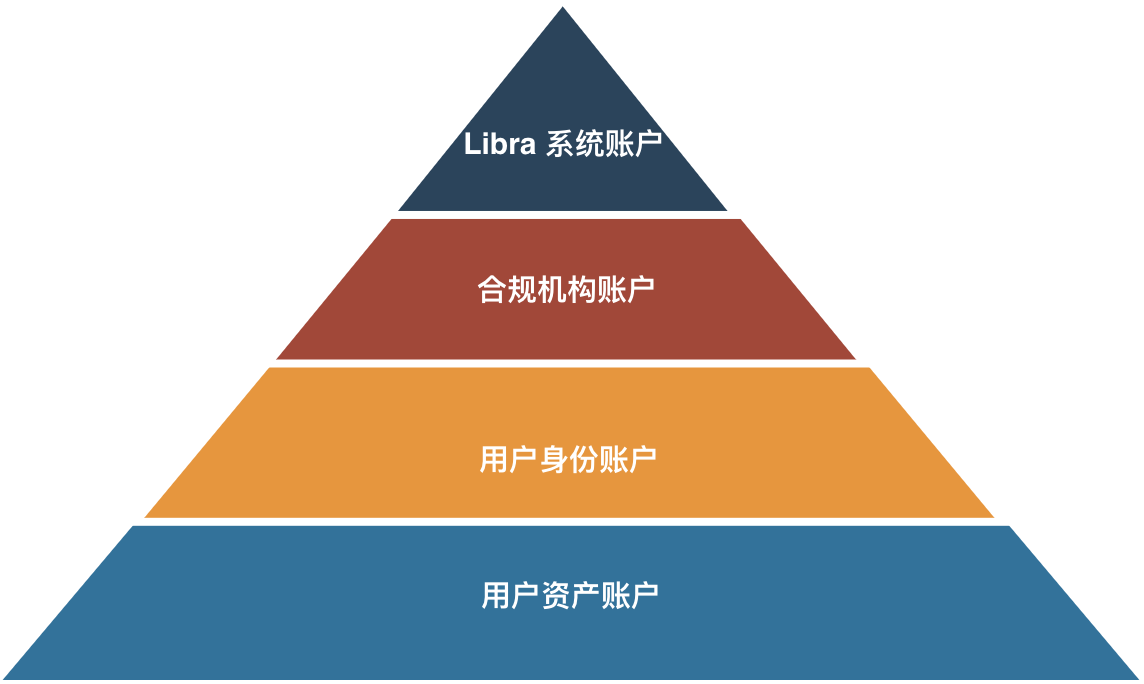
\includegraphics[width=10cm, keepaspectratio]{images/ledger_hierarchy.png}
    \caption{Libra 账户层次结构}
    \label{fig:hierarchy}
\end{figure}

这四种账户形成了一个金字塔结构,下层的账户是由上层的账户创建并且管理的。
第一层的 Libra 系统账户可以视为根账户,从它开始派生出其它所有账户。
第二层的合规机构账户接受 Libra 协会的管理,负责根据本地司法辖区的政策,行使相应的AML/CFT等合规审查职责。
这两种账户都是知名账户,必须公开自己的真实身份,并且接受公众的监督。
第三、四层的账户是 Libra 用户的,无论是个人还是企业,必须接受对应合规机构的管理。
这种分层的账户体系能够帮助 Libra 实现账户的准入、合规和监管等机制,而且能灵活的适应不同司法辖区的差异。
